\section{Das Potenzial-Problem}

Im folgenden werde ich mich mit dem sog. Potential-Problem beschäftigen.

\begin{mydef}
	Das Potential $k$ ist eine Art Kontostand, mit dem eine oder mehrere Kantengewichte reduziert werden können. Die Größe des Potentials gibt an, um wie viel die Gewichte insgesamt reduziert werden dürfen.
\end{mydef}

Ich betrachte verschiedene, unterschiedlich komplizierte Varianten des Potential-Problems und werde für die jeweilige Variante einen Algorithmus angeben und kurz die Laufzeit begründen.

\subsection{Spezialfall $k = 1$}
//TODO algo angeben, wieso ist er liniear? wieso korrekt?
\\
\\
Jeder Knoten berechnet im Algorithmus von BARRIÈRE L. et al. die minimale Anzahl von Agenten (siehe oben) und es lässt sich schnell überlegen, dass die Höhe der Agentenanzahl an jedem Knoten von bestimmten Kanten(-gewichten) abhängt.
\\
\\
Die Idee, um das Potenzial-Problem für den Spezialfall $k = 1$ zu lösen, ist nun, die Abhängigkeiten zu speichern, welche Kante(n) die Agentenzahl in jedem Knoten beeinflusst. Dazu protokollieren wir im Algorithmus (aus Kapitel \ref{modifizierterAlgoChapter}), wie jede berechnete Nachricht zustande kommt, also von welchen Kanten sie abhängt.
\\
\\ 
Wie man in der modifizierten Variante (siehe oben) sehen kann, gibt es drei verschiedene Möglichkeiten, wie eine Nachricht 	$\lambda_{y}$ entstehen kann:

\begin{enumerate}[label=\alph*)]
	
	\item aus den beiden größten Kanten $\lambda_{y} \gets edge_{1} + edge_{2}$ \label{entstehung_nachricht_max1+max2}
	
	\item aus der Kante, über welche die Nachricht gerade verschickt wird (diese entspricht dem Knotengewicht) $\lambda_{y} \gets \omega(x)$
	
	\item aus der größten angekommenen Nachricht $\lambda_{y} \gets l_{1}$

\end{enumerate}

Je nachdem, durch welchen Fall eine Nachricht $\lambda_{y}$ berechnet wird, kommen andere Kanten in Frage, die wir protokollieren müssen.
Allerdings gilt für alle Fälle, dass wir uns maximal zwei Kanten merken müssen, da wir ansonsten die minimale Agentenzahl nicht verringern können. Gibt es mehr als zwei Kanten, so merken wir uns nur die Information, dass es keinen (zwei) eindeutigen Kanten gab bis hierhin (wir setzen einen "flag").

\begin{theorem}
	Wir müssen maximal zwei Kanten pro Nachricht protokollieren. Ansonsten kann das Potential nicht angewendet werden und wir setzen eine "'flag"'
\end{theorem}

\begin{proof}[Widerspruchsbeweis]
	Wir nehmen an, es könnten mehr als zwei Kanten pro Nachricht protokolliert werden, z.B. drei Kanten. Dies würde bedeuten, dass wir durch Reduzierung einer dieser drei Kanten die Nachricht verkleinern könnten. Allerdings hängt die Berechnung der Nachricht pro Fall von maximal zwei Kanten ab (siehe den gerade genannten Fall \ref{entstehung_nachricht_max1+max2}). Wenn also nun eine der drei Kanten reduziert wird, kann sich maximal nur ein Fall verkleinern. Da die drei Kanten aber auf jeden Fall in zwei Fällen auftreten, würde der nicht veränderte Fall die Nachricht nicht verädnern. Da wir aber gesagt haben, dass alle drei Kanten die Nachricht reduzieren ist dies ein Widerspruch, dass eine Nachricht von mehr als zwei Nachrichten abhängt.
\end{proof}

Im folgenden werde ich bei allen drei Fällen von oben beschreiben, welche Kanten unter welcher Bedingung protokolliert werden. Protokollieren bedeutet einfach, dass wir bei der Berechnung der Nachricht $\lambda_{y}$ von x nach y  in die Nachricht mit reinschreiben, welche Kanten diese Nachricht bestimmt haben, bzw. wir protokollieren einen "flag", falls dies mehr als zwei Kanten sind.

\begin{enumerate}[label=\alph*)]
	
	\item In diesem Standardfall wird die Nachricht aus den beiden größten Kanten berechnet (wie oben beschrieben). Allerdings müssen wir kontrollieren, ob diese zwei Kanten eindeutig sind, oder ob es evtl. mehrere gleich große Kanten gibt. Ist die Wahl der Kanten nicht eindeutig, müssen wir dies bei der Protokollierung mit berücksichtigen:\\
	
		\begin{algorithmic}
			\If {$edge_{1} == edge_{3}$}
			\State \uline{protokolliere} "flag"
			\State//Es gibt drei gleich große Kanten. Selbst wenn man eine Kante reduziert, wird die Nachricht aus den anderen beiden Kanten berechnet.
			\ElsIf {$edge_{2} == edge_{3}$}
			\State \uline{protokolliere} $edge_{1}$
			\State//Die maximale Kante ist eindeutig, die zweit größte nicht. Es macht also nur Sinn die größte zu reduzieren.
			\Else
			\State \uline{protokolliere} $edge_{1}$ und $edge_{2}$
			\State//Sowohl die größte, als auch die zweit größte Kante ist eindeutig. Wir können eine von den beiden reduzieren, um auch die Nachricht erfolgreich zu reduzieren.
			\EndIf
		\end{algorithmic}
	
	\item Die Nachricht ist kleiner als das Knotengewicht: $\omega(x) \geq edge_{1}+edge_{2}$. Da aber $\omega(x)$ so definiert ist, dass es den Wert des größten Kantengewicht inzident zu x hat, muss die Kante ausschlaggebend sein, über die die Nachricht verschickt wird. 
	\\
	Diese Kante zwischen x und y ist für den Nachrichtenwert also entscheidend und wird somit in der Nachricht protokolliert: \uline{Protokolliere} Kante zwischen x und y.
	
	\item In diesem Fall bestimmt die größte ankommende Nachricht $l_{1}$ die neu berechnete Nachricht. Da keine weitere Kante mehr Einfluss genommen hat, übernehmen wir die protokollierten Kanten (oder die "flag") aus $l_{1}$ für $\lambda_{y}$: \uline{Protokolliere} das gleiche wie $l_{1}$
	
\end{enumerate}

//TODO alle einzelnen Fälle noch genauer erklären
\\
\\

Man muss noch beachten, dass mehrere Fälle gleichzeitig auftreten können. Passiert dies, muss man einen weiteren Test durchführen, ob die verschiedenen Fälle unterschiedlich protokollieren würden.
\\
Würden die Fälle verschieden protokollieren, so protokolliere "flag", da das Potenzial an dieser Stelle nicht genutzt werden kann, ansonsten behalte die Protokollierung bei.

\subsection{Potenzial auf einer Kante mit k > 1}

Um das Problem des Potenzials etwas zu erweitern, betrachte ich im folgenden Abschnitt Potenziale größer 1, allerdings mit der Einschränkung, dass man das gesamte Potenzial k nur auf einer Kante einsetzen darf.

\begin{theorem}
	Man kann trotz beliebig großen Potential nicht garantieren, dass sich die minimale Anzahl an benötigten Agenten reduziert
\end{theorem}

\begin{proof}[Widerspruchsbeweis]
	Es fällt zunächst auf, dass man nicht garantieren kann, dass sich die Anzahl der benötigten Agenten auf allen Bäumen reduzieren lässt. Hierbei spielt es auch keine Rolle, wie groß das Potenzial k ist, da allein die Eigenschaft, dass man das Potenzial nur auf einer Kante einsetzen kann, genügt, um ein Gegenbeispiel zu finden:
	
	Da das Potenzial k beliebig groß ist, kann man eine Kante auf Kantengewicht 1 setzen, da man dadurch das größtmögliche Potenzial ausnutzt. Trotzdem ist es nicht möglich bei folgendem Baum die Anzahl der Agenten zu reduzieren:
	
	\begin{figure}[h]
		\subfigure[alle Kanten haben Gewicht 4. Alle Knoten benötigen mindestens 8 Agenten.]{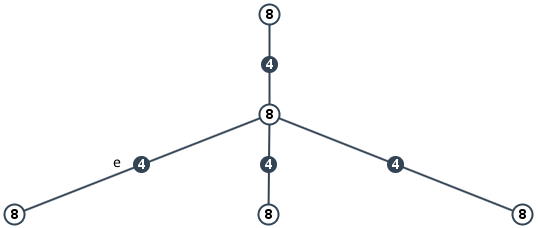
\includegraphics[width=0.49\textwidth]{bilder/abb1.png}} 
		\hfill
		\subfigure[eine Kante wurde auf Gewicht 1 geduziert, alle anderen haben weiterhin Gewicht 4. Alle Knoten benötigen trotzdem mindestens 8 Agenten.]{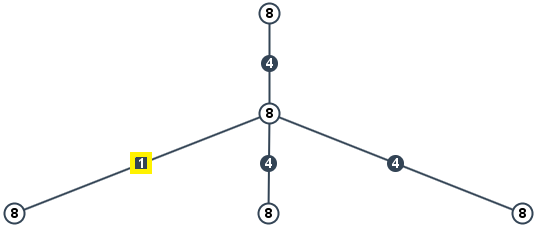
\includegraphics[width=0.49\textwidth]{bilder/abb2.png}} 
		\caption{Beispiel, dass Verringerung auf einer Kante nicht zu einer Verringerung der notwendigen Agenten führen muss} 
	\end{figure} 
\end{proof}

Trotzdem ist es möglich einen Algorithmus anzugeben, der die Kante auswählt, welche die Agentenanzahl am meisten minimiert, falls dies möglich ist.


\subsection*{Algorithmus Idee}

	Auch um dieses Problem werde ich eine Vorschrift angeben, der während des in Kapitel \ref{modifizierterAlgoChapter} beschriebenen Algorithmus Protokoll führt und durch diese Protokollierung am Ende entscheiden kann, welche Kante durch das Potential reduziert werden kann um die Anzahl der Agenten möglichst weit zu reduzieren.\\
	Die Idee ist es für jeden Knoten zwei Dinge festzuhalten: 
	\begin{itemize}
		\item die normale Agentenanzahl (wird wie in Kapitel \ref{modifizierterAlgoChapter} ganz normal berechnet).
		\item die benötigte Anzahl an  Agenten, die durch die maximal mögliche Reduzierung bis zu diesem Zeitpunkt erreicht werden kann, sowie die Kante, die reduziert wurde.
	\end{itemize}
	Hat jeder Knoten am Ende des Algorithmus diese zwei Informationen, kann man mit einem Durchlauf durch alle Knoten das Minimum ermitteln. Da dieses Minimum außerdem die Information hat, welche Kante dafür reduziert werden muss, weiß man, auf welche Kante man das Potential anwendet.
	
	\subsection*{Berechnung der Nachricht}
	
	Um diese Informationen zu generieren, müssen die Nachrichten erweitert werden.
	Diese enthalten nun mehrere Parameter:
	\begin{itemize}
		\item die normal berechnete Nachricht (siehe Kapitel \ref{modifizierterAlgoChapter})
		\item modifizierte Nachricht (,die durch das Potential am stärksten reduzierte Nachricht)
		\item die Kante, auf die das Potential angewendet worden ist
	\end{itemize}
	Es bleibt noch zu klären, wie die modifizierte Nachricht berechnet wird:
	Es gibt mehrere Kanten, auf die das Potential angewendet werden kann um die modifizierte Nachricht zu generieren. Wir müssen auf von allen in frage kommenden Kanten nacheinander das Potential abziehen und dann schauen, wie der Wert der Nachricht mit dieser Kantenreduzierung aussehen würde. Wir merken uns den Fall, bei der diese Reduzierung am stärksten ist und verschicken dies als modifizierte Nachricht. 
	\\
	Wir gehen alle Fälle durch, um die modifizierte Nachricht von Knoten x nach y zu berechnen:
	\begin{enumerate}
		\item betrachte ($edge_{xy} - potential$) und schaue, welchen Wert die Nachricht damit hätte.
		\item betrachte ($edge_{1} - potential$) und schaue, welchen Wert die Nachricht damit hätte.
		\item betrachte ($edge_{2} - potential$) und schaue, welchen Wert die Nachricht damit hätte.
		\item betrachte aus $l_{1}$ nicht die normale Nachricht, sondern die modifizierte Nachricht und schaue, welchen Wert die Nachricht damit hätte.
	\end{enumerate}
	Der kleinste Wert aus diesen Punkten ist unsere modifizierte Nachricht. Die Kante, auf die das Potential angewendet wurde, wird als 3. Parameter in der Nachricht mit verschickt.
	

TODO:\\
//überlegung: woran sieht man, ob man die Agentenanzahl verringern kann?\\
//algorithmus angeben, welche kante ausgesucht wird?\\
//linear

\subsection{Potenzial verteilen mit k > 1}